\chapter{Experiments}\label{experiments}

The purpose of the application is to speed up the computation process.
Thus it should be verified, whether the improvement makes sense or do
not. The improvement should correspond to the number of nodes involved
in the computation. Our wish is, that the dependence is of some linear
form, that is, the computation gets faster with every additional node
and it improves by the same steps. In this hypothetical ideal case two
nodes means two times faster computation and one hundred nodes means one
hundred times faster achievement of the result. However, this is
impossible for several reasons. At first, we must consider time that is
taken by the division process. Additional time is consumed by the
transfers and final join operation. Another problem arises from the
fact, that the transfers are quite demanding themselves. So when more
transfers are ongoing at a particular moment, the initiator is more
utilized and the process can be slowed down due to this fact. This also
implies that the improvement does not raise linearly when adding more
nodes. Finally, we must consider delays which can appear due to
technical reasons, network congestion or node failures.

\section{Approach to testing}\label{approach-to-testing}

If we want to obtain reasonable data, the measurements must be repeated
several times to prevent deviations. Also we want to keep the
measurements independent to make its statistical processing easier. Our
approach to the testing and gathering results is described in this
chapter. Our main goal is to measure the improvement, but we would also
like to measure the impact of the particular setting on the result.

The tests were run in the school laboratory. The network consists of
several computers connected together with common ethernet twisted pair
cables. Each computer has currently installed 64 bit Gentoo
Linux\footnote{https://www.gentoo.org/} with the Linux kernel version
3.18. The machines are equipped with Intel Core i7 processors and 6 GB
of operation memory. The
MTU\footnote{https://en.wikipedia.org/wiki/Maximum\_Transmission\_Unit}
is set to 1500B and the network uses Gigabit
Ethernet\footnote{https://en.wikipedia.org/wiki/Ethernet}.

Because of the number of tests, it is desirable for the testing process
to be automated. Special Bash script was created for this reason. The
script is tailored to be used at the testing laboratory, so it may need
little modifications to work in some different environment. It is
distributed with the source code of the framework. To allow automated
and robust execution of the tests, special functionality was added to
the program. It is invokable by option given at the start time and
causes the program to run in a non-interactive mode. No input is
accepted in this mode, the program just processes given file and ends.
This options assumes all the essential data are given at the start time
of the program. To keep the measurements independent, all the instances
(on every node) of the program are started when the test begins and they
are killed in the end. Communication with the remote nodes is handled by
the ssh program\footnote{https://en.wikipedia.org/wiki/Secure\_Shell}.
The testing script uses a special file which describes the particular
run. Working example of such file together with explanations of the
values is given below.

\begin{samepage}
\begin{verbatim}
v6 // use IPv6
/afs/ms/u/h/hudecekv/futu.avi // location of the file to be re-encoded
2 // run the whole scenario twice
slower // quality of the encoding
10000 // chunk size [KByte]
2048576 // transfer buffer size
spawn u-pl1 2221 // spawn the program on the machine 'u-pl1', use port 2221
spawn u-pl2 2222
spawn u-pl4 2224
spawn u-pl5 2225
spawn u-pl6 2226
spawn u-pl7 2227
wait 10 // wait for ten seconds before next action
kill u-pl4 // kill the instance of program running on machine 'u-pl4'
spawn u-pl8 2228
spawn u-pl9 2229
spawn u-pl10 2230
\end{verbatim}
\end{samepage}

Thanks to this mechanism, various scenarios can be run easily without
the need of human interaction.

The data were collected by running each test ten times for the given
configuration. The count of involved nodes varied from one to ten. Each
test was run once with chunks of 40 000 kB in size and once with 10 000
kB chunks. The same file was used each time as well as the encoding
quality. The sample input file was packed in the \textit{avi} container,
encoded with the \textit{msmpeg} codec. It was re-encoded with
\textit{H264} codec and stored in the \textit{mkv} container. Each test
gathered various results, among others the average times needed for
transfer and encoding, number of chunks, quality and count of involved
nodes. Because we had not the chance to run the tests in some dedicated
network, the computation times may vary for the given settings. It
depends on the conditions during the test. This is obviously a problem,
because we can't compare such results. The tests showed, that if we
multiply the average time needed to encode one chunk by the count of
chunks, the product corresponds to the time that the serial encoding
process would take. This allows us to deal with the problem, because we
can use this computed estimation to obtain the improvement and the error
will be minimal.

The desired values have been gathered in two ways. Some of them, for
example average transfer and encoding times, are measured directly in
the program and then outputted to a special file. The testing script
just reads it from this file. The rest of the values is measured by the
script.

\section{Results}\label{results}

\subsection{Interpreting the results}\label{interpreting-the-results}

In the Figure 3.1 are showed the achieved results, interpreted with
respect to time needed by the single node. The x-axis shows count of
nodes, the y-axis the portion of time needed by the distributed process.
The blue dashed line represents the estimate which is based on the model
which used hyperbolic function to predict the data. The obtained data
are visualized as black crosses, red squares show respective mean
values.

\begin{figure}[h]
\begin{center}
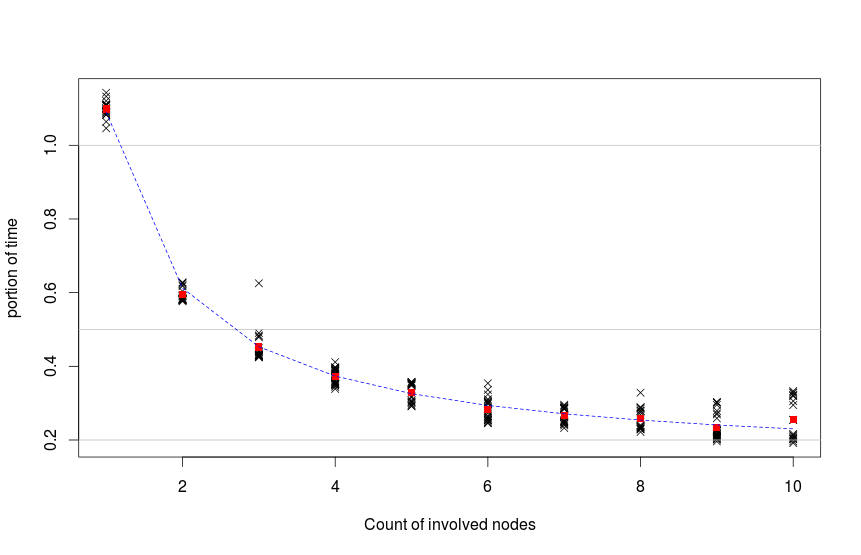
\includegraphics[scale=0.45]{./img/improvement_root.png}
\caption{Achieved improvement - all measurements}
\end{center}
\end{figure}

The figures 3.2 - 3.4 shows the achieved speedup. The y-axis shows the
obtained speedup. Model that was used is further described in the next
section. The data are represented by gray crosses, the estimation based
on the model is visualized by the blue dashed line. The red line shows
the linear function, which would be the ideal case. This linear function
is of the form

\begin{center}
$y = q*x$
\end{center}

where coefficient \textit{q} represents the influence of the time
consumed by the data transfers. The Figure 3.4 shows, that for this
chunk size the time spent with the distribution causes latency when more
nodes are employed. This is caused by the fact, that too many transfers
are processed in parallel. Consequently, some of the nodes have to wait
for the chunks for too long.

\begin{figure}[h]
\begin{center}
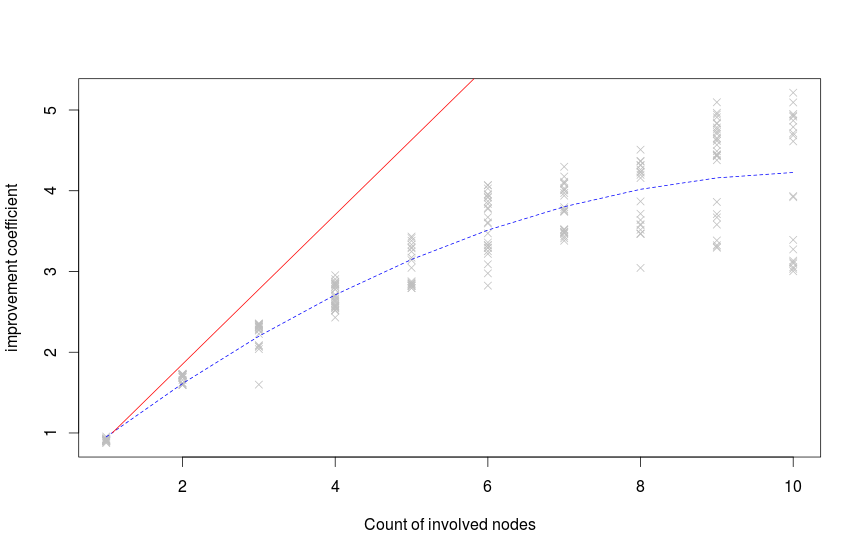
\includegraphics[scale=0.45]{./img/Rplot_all.png}
\caption{Achieved speedup - all measurements}
\end{center}
\end{figure}

\begin{figure}[h]
\begin{center}
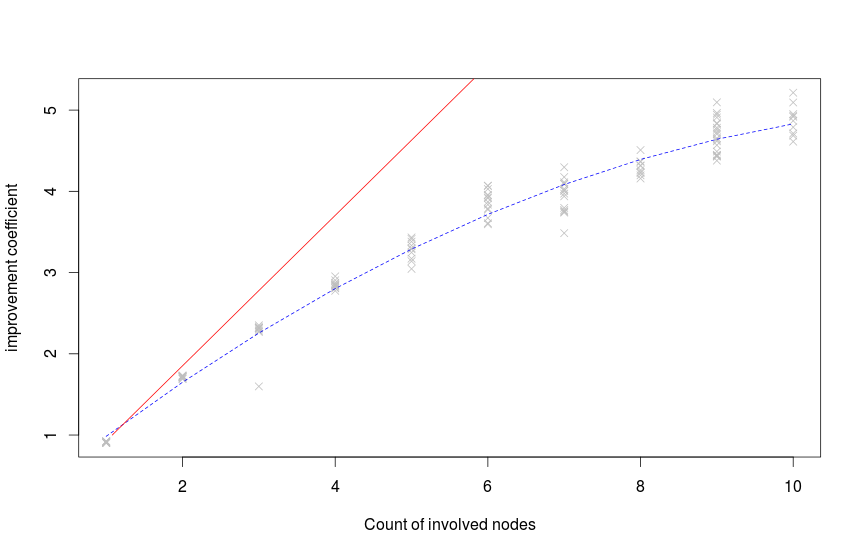
\includegraphics[scale=0.45]{./img/Rplot10k.png}
\caption{Achieved speedup - 10 MB chunks}
\end{center}
\end{figure}

\begin{figure}[h]
\begin{center}
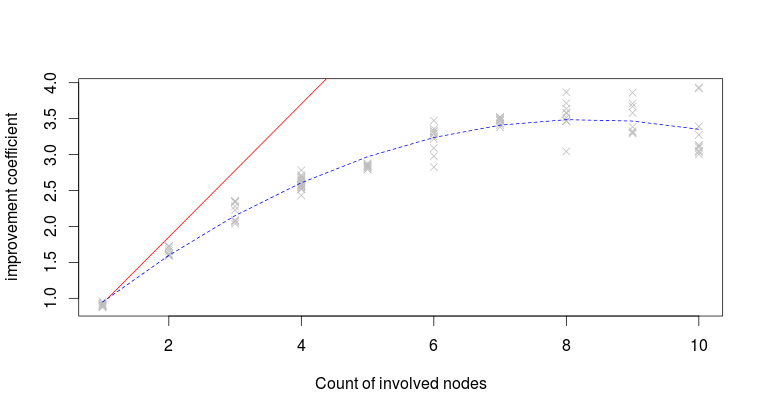
\includegraphics[scale=0.45]{./img/Rplot40k.png}
\caption{Achieved speedup - 40 MB chunks}
\end{center}
\end{figure}

In the Figures 3.5 and 3.6 are displayed ratios between particular
operations performed during the process. The ratios are displayed with
respect to the time that would be taken by the serial execution. Each
column represents one measurement (process). The first image displays
data for chunks with 10 MB in size, the second shows 40 MB chunks. The
data are sorted according to the number of neighbors used in the
process. We can see that portion of time spent with network transfers is
relatively small in our case. These charts were generated using the
LibreOffice package\footnote{http://www.libreoffice.org/}

\begin{figure}[h]
\begin{center}
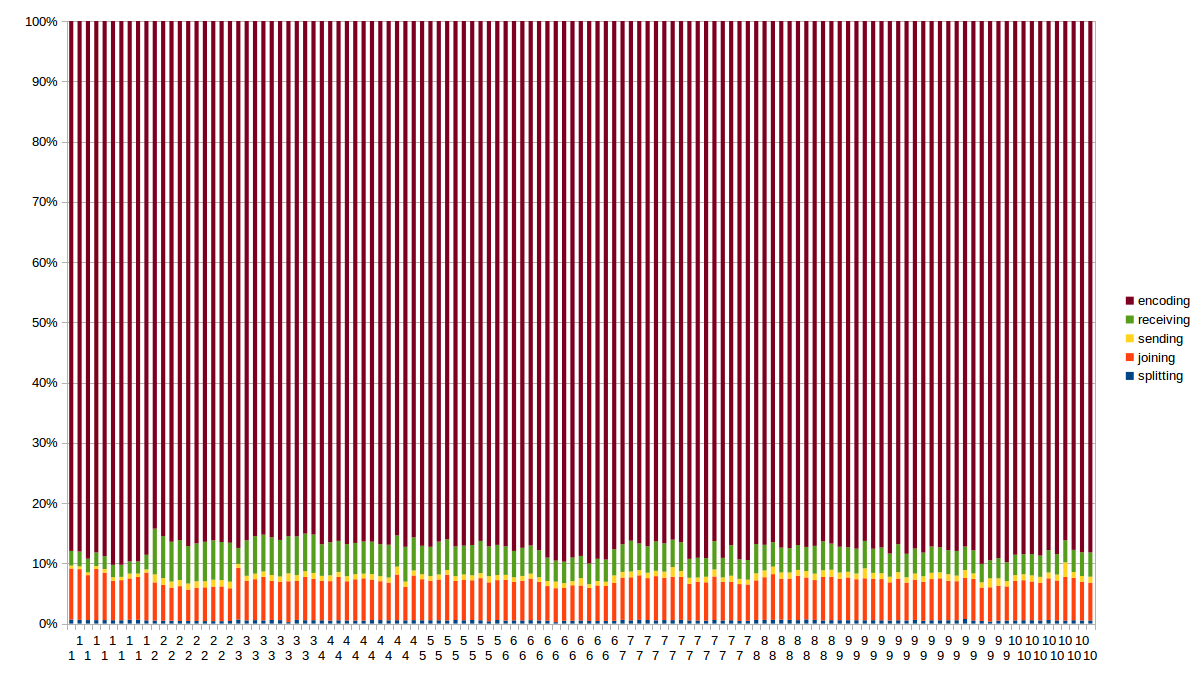
\includegraphics[scale=0.5]{./img/comparison_chart.png}
\caption{Comparison of operation times - 10 MB chunks}
\end{center}
\end{figure}

\begin{figure}[h]
\begin{center}
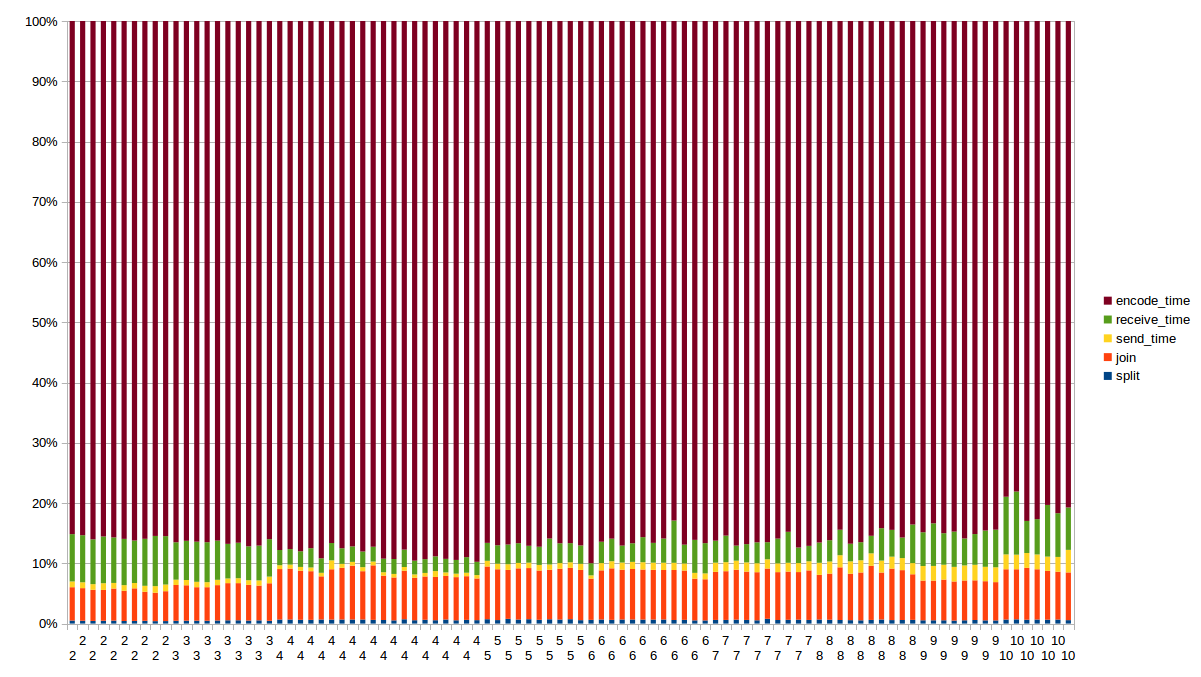
\includegraphics[scale=0.5]{./img/comparison_chart40k.png}
\caption{Comparison of operation times - 40 MB chunks}
\end{center}
\end{figure}

Figure 3.7 shows results of the experiment, in which one of the nodes
was killed during the process and then spawned again. As a result,
several chunks were sent more times, depending on the conditions in the
network. The plot shows average number of chunk sent and achieved
improvement. In this experiment, 40 MB chunks were used, displayed in
the left side. Also, some of the experiments were intentionally run with
no failure, so we can see results achieved with normal run in the left
down corner and we can compare it. Those values are highlighted. We can
see, that resending of chunks has great impact on the result. This
problem could be reduced by using smaller chunks. When we used 5 MB
chunks, the results improved significantly as showed in the right image
in the Figure. This is caused by the fact, that with the same number of
faults, the amount of work that needs to be done again is smaller when
using smaller chunks. However, disadvantage of this approach is, that
the split and join operations take slightly more time.

\begin{figure}[h]
\begin{center}
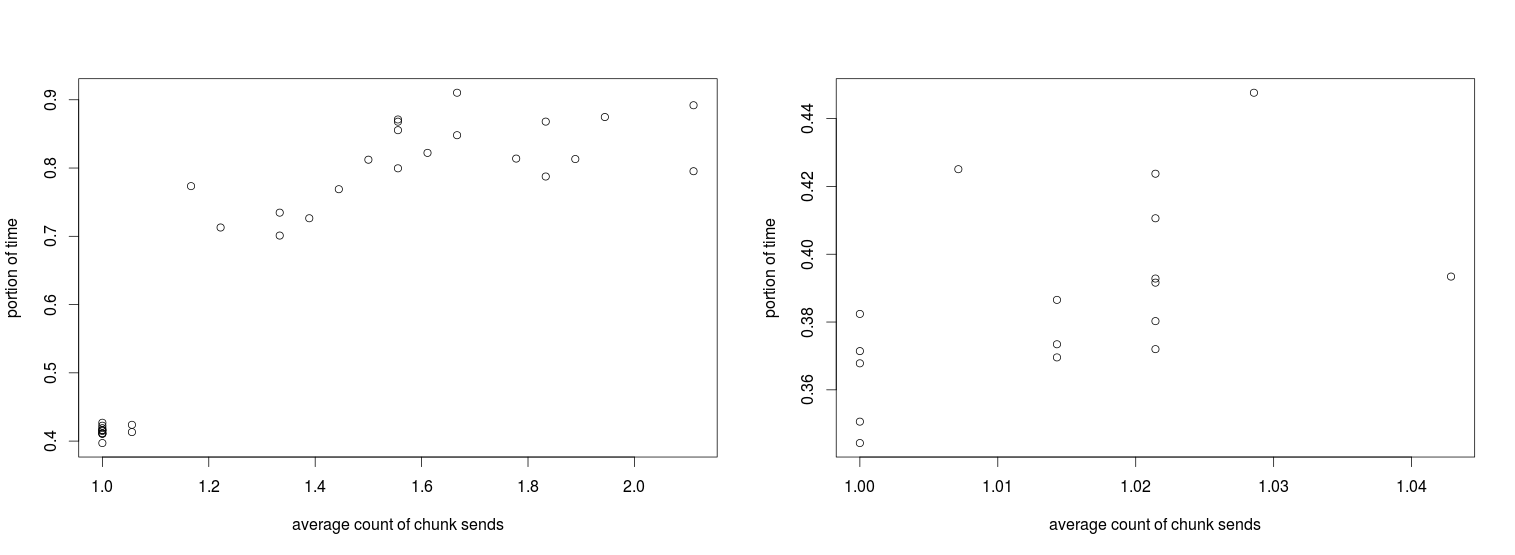
\includegraphics[scale=0.30]{./img/failures_both.png}
\caption{Impact of resending on the result}
\end{center}
\end{figure}

\pagebreak

\subsection{Linear Model}\label{linear-model}

Work with the data and the model was performed in the R Studio
program\footnote{https://www.rstudio.com/}. To evaluate the data, simple
linear regression model was used. Specifically, subsequent formula was
used:

\begin{center}
$\frac{single\_node\_time}{distributed\_time} = \beta_0 + \beta_1 \times neighbor\_count + \beta_2 \times neighbor\_count^2 + \epsilon_i$
\end{center}

Higher powers were not used in order to not over fit the model. The
analysis of the model showed, that it makes sense to use this model. The
assumptions such as homoscedasticity (constant variance) and
independence of errors were explored using plots and results given by
the R Studio. Some of the mentioned outputs are given in the Figures 3.8
and 3.9. We can see, that according to the p-values corresponding to
coefficients, all of them are significant for the model. Residual
standard error shows, that the variance is not too big. In the plots we
can see that the residuals unfortunately has not constant variance. The
second plot also suggests, that they probably are not distributed
normally. However, citation says: ``heteroscedasticity has never been a
reason to throw out an otherwise good model.''\citep{ECON} So we used
this model in our modeling. It may be questionable, whether we had
enough measurements, however, the model seems to be good enough to
describe the data and predict the behavior for more nodes. We can also
notice, that the $\beta_2$ coefficient is negative and since the squared
value rises faster, there is some point at which the improvement stops
raising, which corresponds to reality.

\begin{figure}[h]
\begin{center}
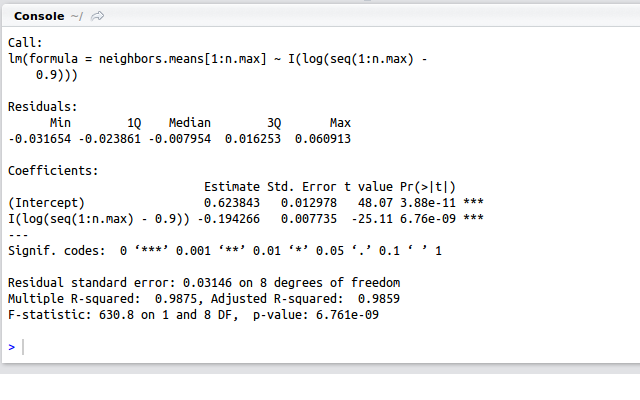
\includegraphics[scale=0.60]{./img/model.png}
\caption{Summary of the model}
\end{center}
\end{figure}

\begin{figure}[h]
\begin{center}
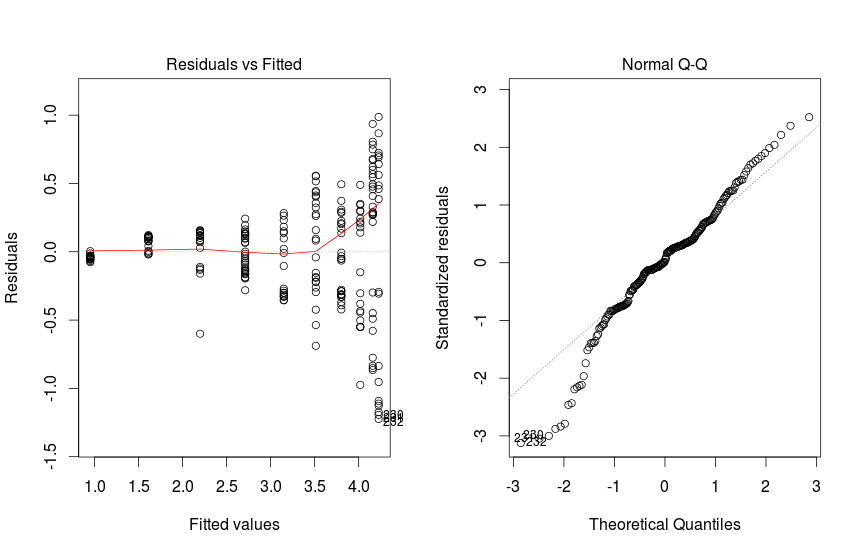
\includegraphics[scale=0.45]{./img/model_plots.png}
\caption{Graphical representation of the model data}
\end{center}
\end{figure}

\subsection{Upper Bounds}\label{upper-bounds}

Overall time of the process can be divided into operations split, send,
encode, receive and join (in this order). It is also influenced by
searching appropriate neighbors, but it will not be taken into account
in this analysis. Also, based on the data we can observe, that the time
taken by the split operation is not very significant, therefore we can
omit it. If we ask how big speedup can be achieved, we can use the
Amdahl's law\footnote{https://en.wikipedia.org/wiki/Amdahl's\_law} to
model the situation. The join operation can not be parallelized. The
encoding itself is parallelized completely. The data transfer operations
are performed theoretically in parallel, however, in practice we are
limited by the network throughput and the system resources of the
initiator, i.e.~how many data transfers it can handle in parallel. This
can be influenced by the OS, disk speed or even operation memory.
Because this number is limited, the initiator can not employ arbitrary
number of nodes effectively. If we want to deal with this problem, we
have to consider several facts. The speed of the distribution is
influenced by the ability of the nodes to receive the data with no
delay, so we assume that buffering and disk operations do not slow down
the process. Also, the full network capacity cannot be used because of
other ongoing transfers. Some portion of the capacity is consumed by the
redundant information used by the TCP/IP too. For the sake of
simplicity, we will make the assumption, that the capacity corresponds
to the actual amount of useful data transfered. We also must not forgot,
that the sizes of original and received chunks differs. Finally, we
treat the parallel transfer over the network as it took the same time as
the serial, which does not have to be always true. We will consider the
size of received chunks to be $k$ times bigger than the size of the send
ones and count with this size. Let $c$ be the amount of data that can be
transfered over the network per one second, $s$ chunk size and $t$ time
needed to encode one chunk (here we assume the encoding times are the
same for all the nodes). Then maximum number $n$ of effectively employed
nodes must fulfill the inequality:

\begin{center}
$\frac{n \times s}{c} \leq t$
\end{center}

since otherwise the transfer would take more time than the encoding, so
the encoded chunks would have to wait.

To applicate the Amdahl's law, we must determine the fraction of the
algorithm that is strictly serial. This involves the splitting and
joining. We consider the data transfers to be parallelized with the
preceding paragraph in mind. According to the results, the split and
join operations take approximately 7.5\% of time in average. So
according to the basic form of the law, the theoretical maximum speedup
should be obtained from the following formula:

\begin{center}
$S=\lim_{n \to +\infty} \frac{1}{B + \frac{1}{n}(1 - B)} = \frac{1}{B} = \frac{1}{0.075} = 13.33$
\end{center}

Where $B$ represents the serial fraction. This result is strictly
theoretical and does not correspond to real situation, mainly because of
the problems mentioned above. We can obtain more realistic results by
using the formula to estimate the parallel fraction of time.

\begin{center}
$P_{est} = \frac{\frac{1}{speedup}-1}{\frac{1}{node count} - 1}$
\end{center}

For our data the estimation equals $0.89$, which gives us theoretical
maximum speedup $9.09$.
